\documentclass[12pt,a4paper,fleqn]{article}
\title{Progress Report}
\author{Syed Ahmad Raza}
\date{2016.11.15}
\usepackage{amsmath}
\usepackage{graphicx}
\usepackage{color}			% for color eps output

\begin{document}
	\maketitle
		\section*{First order numerical differentiation}
		An algorithm was coded in C++ for numerical differentiation using three different commonly used schemes. The functions sin$(3x)$ and cos$(3x)$ were differentiated using forward difference method, backward difference method and central difference method.
		
			\subsection*{Forward difference method}
			\begin{equation}
			f^\prime(x) = \frac{f(x_{i+1})-f(x_i)}{x_{i+1}-x_i}
			\end{equation}
			
			\subsection*{Backward difference method}
			\begin{equation}
			f^\prime(x) = \frac{f(x_i)-f(x_{i-1})}{x_i-x_{i-1}}
			\end{equation}
			
			\subsection*{Central difference method}
			\begin{equation}
			f^\prime(x) = \frac{f(x_{i+1})-f(x_{i-1})}{x_{i+1}-x_{i-1}}
			\end{equation}
		
		The results are shown in the figures below.
		\begin{figure}
			\centering
			% GNUPLOT: LaTeX picture with Postscript
\begingroup
  \makeatletter
  \providecommand\color[2][]{%
    \GenericError{(gnuplot) \space\space\space\@spaces}{%
      Package color not loaded in conjunction with
      terminal option `colourtext'%
    }{See the gnuplot documentation for explanation.%
    }{Either use 'blacktext' in gnuplot or load the package
      color.sty in LaTeX.}%
    \renewcommand\color[2][]{}%
  }%
  \providecommand\includegraphics[2][]{%
    \GenericError{(gnuplot) \space\space\space\@spaces}{%
      Package graphicx or graphics not loaded%
    }{See the gnuplot documentation for explanation.%
    }{The gnuplot epslatex terminal needs graphicx.sty or graphics.sty.}%
    \renewcommand\includegraphics[2][]{}%
  }%
  \providecommand\rotatebox[2]{#2}%
  \@ifundefined{ifGPcolor}{%
    \newif\ifGPcolor
    \GPcolortrue
  }{}%
  \@ifundefined{ifGPblacktext}{%
    \newif\ifGPblacktext
    \GPblacktextfalse
  }{}%
  % define a \g@addto@macro without @ in the name:
  \let\gplgaddtomacro\g@addto@macro
  % define empty templates for all commands taking text:
  \gdef\gplbacktext{}%
  \gdef\gplfronttext{}%
  \makeatother
  \ifGPblacktext
    % no textcolor at all
    \def\colorrgb#1{}%
    \def\colorgray#1{}%
  \else
    % gray or color?
    \ifGPcolor
      \def\colorrgb#1{\color[rgb]{#1}}%
      \def\colorgray#1{\color[gray]{#1}}%
      \expandafter\def\csname LTw\endcsname{\color{white}}%
      \expandafter\def\csname LTb\endcsname{\color{black}}%
      \expandafter\def\csname LTa\endcsname{\color{black}}%
      \expandafter\def\csname LT0\endcsname{\color[rgb]{1,0,0}}%
      \expandafter\def\csname LT1\endcsname{\color[rgb]{0,1,0}}%
      \expandafter\def\csname LT2\endcsname{\color[rgb]{0,0,1}}%
      \expandafter\def\csname LT3\endcsname{\color[rgb]{1,0,1}}%
      \expandafter\def\csname LT4\endcsname{\color[rgb]{0,1,1}}%
      \expandafter\def\csname LT5\endcsname{\color[rgb]{1,1,0}}%
      \expandafter\def\csname LT6\endcsname{\color[rgb]{0,0,0}}%
      \expandafter\def\csname LT7\endcsname{\color[rgb]{1,0.3,0}}%
      \expandafter\def\csname LT8\endcsname{\color[rgb]{0.5,0.5,0.5}}%
    \else
      % gray
      \def\colorrgb#1{\color{black}}%
      \def\colorgray#1{\color[gray]{#1}}%
      \expandafter\def\csname LTw\endcsname{\color{white}}%
      \expandafter\def\csname LTb\endcsname{\color{black}}%
      \expandafter\def\csname LTa\endcsname{\color{black}}%
      \expandafter\def\csname LT0\endcsname{\color{black}}%
      \expandafter\def\csname LT1\endcsname{\color{black}}%
      \expandafter\def\csname LT2\endcsname{\color{black}}%
      \expandafter\def\csname LT3\endcsname{\color{black}}%
      \expandafter\def\csname LT4\endcsname{\color{black}}%
      \expandafter\def\csname LT5\endcsname{\color{black}}%
      \expandafter\def\csname LT6\endcsname{\color{black}}%
      \expandafter\def\csname LT7\endcsname{\color{black}}%
      \expandafter\def\csname LT8\endcsname{\color{black}}%
    \fi
  \fi
    \setlength{\unitlength}{0.0500bp}%
    \ifx\gptboxheight\undefined%
      \newlength{\gptboxheight}%
      \newlength{\gptboxwidth}%
      \newsavebox{\gptboxtext}%
    \fi%
    \setlength{\fboxrule}{0.5pt}%
    \setlength{\fboxsep}{1pt}%
\begin{picture}(7766.00,7766.00)%
    \gplgaddtomacro\gplbacktext{%
      \csname LTb\endcsname%
      \put(682,704){\makebox(0,0)[r]{\strut{}$-3$}}%
      \put(682,1837){\makebox(0,0)[r]{\strut{}$-2$}}%
      \put(682,2970){\makebox(0,0)[r]{\strut{}$-1$}}%
      \put(682,4102){\makebox(0,0)[r]{\strut{}$0$}}%
      \put(682,5235){\makebox(0,0)[r]{\strut{}$1$}}%
      \put(682,6368){\makebox(0,0)[r]{\strut{}$2$}}%
      \put(682,7501){\makebox(0,0)[r]{\strut{}$3$}}%
      \put(814,484){\makebox(0,0){\strut{}$0$}}%
      \put(2453,484){\makebox(0,0){\strut{}$\pi/4$}}%
      \put(4091,484){\makebox(0,0){\strut{}$\pi/2$}}%
      \put(5730,484){\makebox(0,0){\strut{}$3\pi/4$}}%
      \put(7369,484){\makebox(0,0){\strut{}$\pi$}}%
    }%
    \gplgaddtomacro\gplfronttext{%
      \csname LTb\endcsname%
      \put(176,4102){\rotatebox{-270}{\makebox(0,0){\strut{}$f(x)$}}}%
      \put(4091,154){\makebox(0,0){\strut{}$x$}}%
      \csname LTb\endcsname%
      \put(5471,1727){\makebox(0,0)[r]{\strut{}Forward}}%
      \csname LTb\endcsname%
      \put(5471,1507){\makebox(0,0)[r]{\strut{}Backward}}%
      \csname LTb\endcsname%
      \put(5471,1287){\makebox(0,0)[r]{\strut{}Central}}%
      \csname LTb\endcsname%
      \put(5471,1067){\makebox(0,0)[r]{\strut{}Analytical}}%
    }%
    \gplbacktext
    \put(0,0){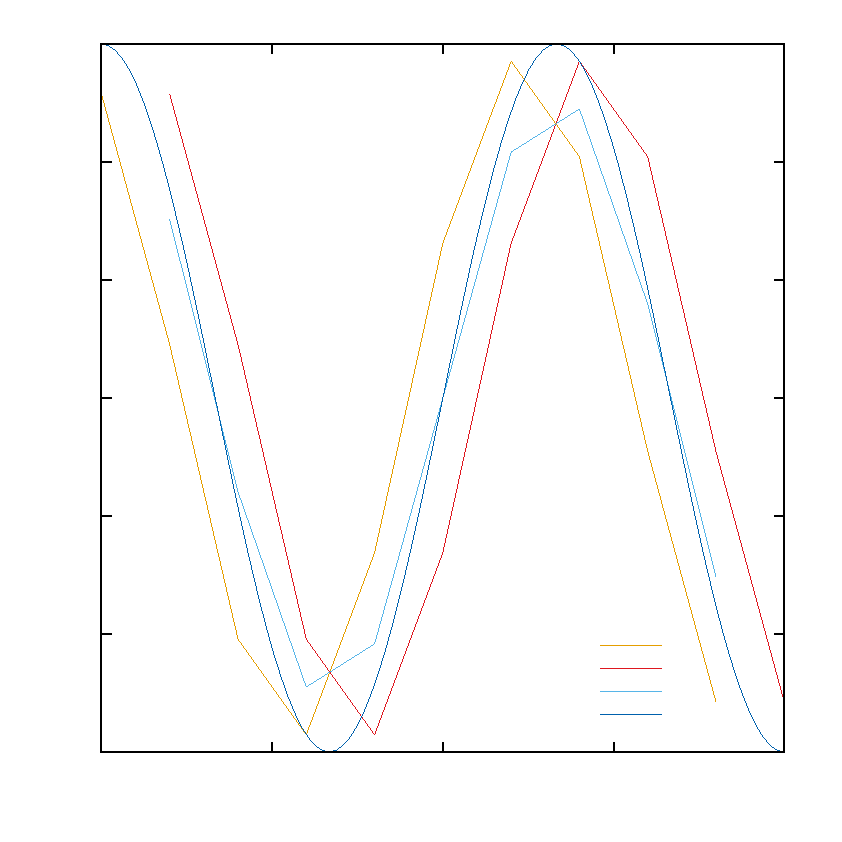
\includegraphics{1stsin10}}%
    \gplfronttext
  \end{picture}%
\endgroup

			\caption{Comparison of numerical differentiation of sin$(3x)$ using 10 intervals}
		\end{figure}
		\begin{figure}
			\centering
			% GNUPLOT: LaTeX picture with Postscript
\begingroup
  \makeatletter
  \providecommand\color[2][]{%
    \GenericError{(gnuplot) \space\space\space\@spaces}{%
      Package color not loaded in conjunction with
      terminal option `colourtext'%
    }{See the gnuplot documentation for explanation.%
    }{Either use 'blacktext' in gnuplot or load the package
      color.sty in LaTeX.}%
    \renewcommand\color[2][]{}%
  }%
  \providecommand\includegraphics[2][]{%
    \GenericError{(gnuplot) \space\space\space\@spaces}{%
      Package graphicx or graphics not loaded%
    }{See the gnuplot documentation for explanation.%
    }{The gnuplot epslatex terminal needs graphicx.sty or graphics.sty.}%
    \renewcommand\includegraphics[2][]{}%
  }%
  \providecommand\rotatebox[2]{#2}%
  \@ifundefined{ifGPcolor}{%
    \newif\ifGPcolor
    \GPcolortrue
  }{}%
  \@ifundefined{ifGPblacktext}{%
    \newif\ifGPblacktext
    \GPblacktextfalse
  }{}%
  % define a \g@addto@macro without @ in the name:
  \let\gplgaddtomacro\g@addto@macro
  % define empty templates for all commands taking text:
  \gdef\gplbacktext{}%
  \gdef\gplfronttext{}%
  \makeatother
  \ifGPblacktext
    % no textcolor at all
    \def\colorrgb#1{}%
    \def\colorgray#1{}%
  \else
    % gray or color?
    \ifGPcolor
      \def\colorrgb#1{\color[rgb]{#1}}%
      \def\colorgray#1{\color[gray]{#1}}%
      \expandafter\def\csname LTw\endcsname{\color{white}}%
      \expandafter\def\csname LTb\endcsname{\color{black}}%
      \expandafter\def\csname LTa\endcsname{\color{black}}%
      \expandafter\def\csname LT0\endcsname{\color[rgb]{1,0,0}}%
      \expandafter\def\csname LT1\endcsname{\color[rgb]{0,1,0}}%
      \expandafter\def\csname LT2\endcsname{\color[rgb]{0,0,1}}%
      \expandafter\def\csname LT3\endcsname{\color[rgb]{1,0,1}}%
      \expandafter\def\csname LT4\endcsname{\color[rgb]{0,1,1}}%
      \expandafter\def\csname LT5\endcsname{\color[rgb]{1,1,0}}%
      \expandafter\def\csname LT6\endcsname{\color[rgb]{0,0,0}}%
      \expandafter\def\csname LT7\endcsname{\color[rgb]{1,0.3,0}}%
      \expandafter\def\csname LT8\endcsname{\color[rgb]{0.5,0.5,0.5}}%
    \else
      % gray
      \def\colorrgb#1{\color{black}}%
      \def\colorgray#1{\color[gray]{#1}}%
      \expandafter\def\csname LTw\endcsname{\color{white}}%
      \expandafter\def\csname LTb\endcsname{\color{black}}%
      \expandafter\def\csname LTa\endcsname{\color{black}}%
      \expandafter\def\csname LT0\endcsname{\color{black}}%
      \expandafter\def\csname LT1\endcsname{\color{black}}%
      \expandafter\def\csname LT2\endcsname{\color{black}}%
      \expandafter\def\csname LT3\endcsname{\color{black}}%
      \expandafter\def\csname LT4\endcsname{\color{black}}%
      \expandafter\def\csname LT5\endcsname{\color{black}}%
      \expandafter\def\csname LT6\endcsname{\color{black}}%
      \expandafter\def\csname LT7\endcsname{\color{black}}%
      \expandafter\def\csname LT8\endcsname{\color{black}}%
    \fi
  \fi
    \setlength{\unitlength}{0.0500bp}%
    \ifx\gptboxheight\undefined%
      \newlength{\gptboxheight}%
      \newlength{\gptboxwidth}%
      \newsavebox{\gptboxtext}%
    \fi%
    \setlength{\fboxrule}{0.5pt}%
    \setlength{\fboxsep}{1pt}%
\begin{picture}(7766.00,7766.00)%
    \gplgaddtomacro\gplbacktext{%
      \csname LTb\endcsname%
      \put(682,704){\makebox(0,0)[r]{\strut{}$-3$}}%
      \put(682,1837){\makebox(0,0)[r]{\strut{}$-2$}}%
      \put(682,2970){\makebox(0,0)[r]{\strut{}$-1$}}%
      \put(682,4102){\makebox(0,0)[r]{\strut{}$0$}}%
      \put(682,5235){\makebox(0,0)[r]{\strut{}$1$}}%
      \put(682,6368){\makebox(0,0)[r]{\strut{}$2$}}%
      \put(682,7501){\makebox(0,0)[r]{\strut{}$3$}}%
      \put(814,484){\makebox(0,0){\strut{}$0$}}%
      \put(2453,484){\makebox(0,0){\strut{}$\pi/4$}}%
      \put(4091,484){\makebox(0,0){\strut{}$\pi/2$}}%
      \put(5730,484){\makebox(0,0){\strut{}$3\pi/4$}}%
      \put(7369,484){\makebox(0,0){\strut{}$\pi$}}%
    }%
    \gplgaddtomacro\gplfronttext{%
      \csname LTb\endcsname%
      \put(176,4102){\rotatebox{-270}{\makebox(0,0){\strut{}$f(x)$}}}%
      \put(4091,154){\makebox(0,0){\strut{}$x$}}%
      \csname LTb\endcsname%
      \put(5471,1727){\makebox(0,0)[r]{\strut{}Forward}}%
      \csname LTb\endcsname%
      \put(5471,1507){\makebox(0,0)[r]{\strut{}Backward}}%
      \csname LTb\endcsname%
      \put(5471,1287){\makebox(0,0)[r]{\strut{}Central}}%
      \csname LTb\endcsname%
      \put(5471,1067){\makebox(0,0)[r]{\strut{}Analytical}}%
    }%
    \gplbacktext
    \put(0,0){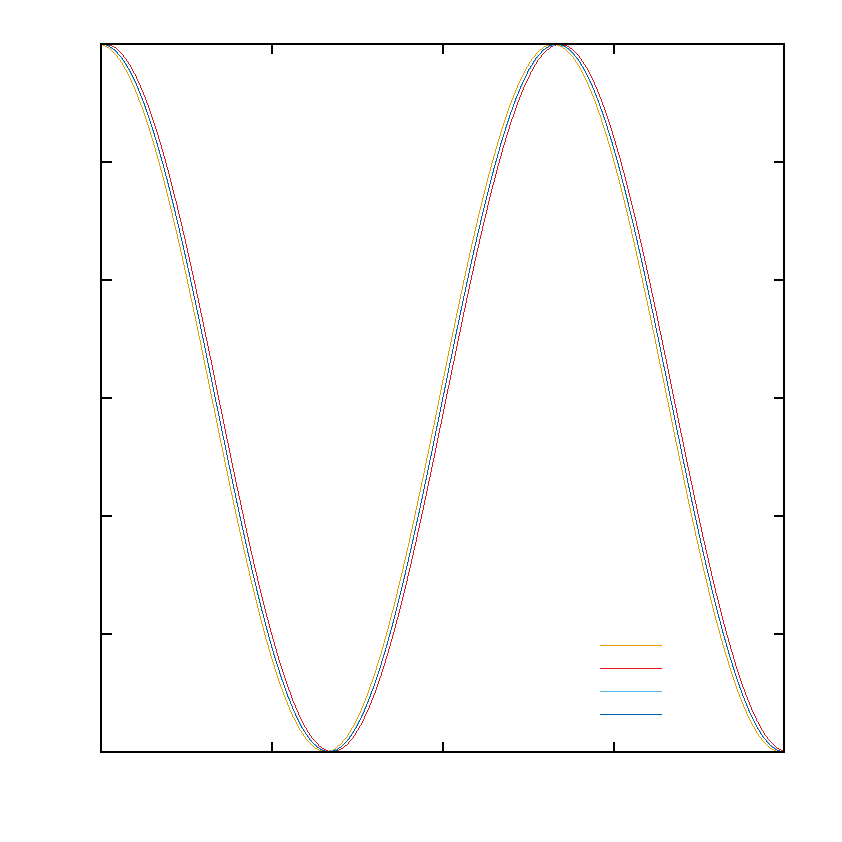
\includegraphics{1stsin100}}%
    \gplfronttext
  \end{picture}%
\endgroup

			\caption{Comparison of numerical differentiation of sin$(3x)$ using 100 intervals}
		\end{figure}
		\begin{figure}
			\centering
			% GNUPLOT: LaTeX picture with Postscript
\begingroup
  \makeatletter
  \providecommand\color[2][]{%
    \GenericError{(gnuplot) \space\space\space\@spaces}{%
      Package color not loaded in conjunction with
      terminal option `colourtext'%
    }{See the gnuplot documentation for explanation.%
    }{Either use 'blacktext' in gnuplot or load the package
      color.sty in LaTeX.}%
    \renewcommand\color[2][]{}%
  }%
  \providecommand\includegraphics[2][]{%
    \GenericError{(gnuplot) \space\space\space\@spaces}{%
      Package graphicx or graphics not loaded%
    }{See the gnuplot documentation for explanation.%
    }{The gnuplot epslatex terminal needs graphicx.sty or graphics.sty.}%
    \renewcommand\includegraphics[2][]{}%
  }%
  \providecommand\rotatebox[2]{#2}%
  \@ifundefined{ifGPcolor}{%
    \newif\ifGPcolor
    \GPcolortrue
  }{}%
  \@ifundefined{ifGPblacktext}{%
    \newif\ifGPblacktext
    \GPblacktextfalse
  }{}%
  % define a \g@addto@macro without @ in the name:
  \let\gplgaddtomacro\g@addto@macro
  % define empty templates for all commands taking text:
  \gdef\gplbacktext{}%
  \gdef\gplfronttext{}%
  \makeatother
  \ifGPblacktext
    % no textcolor at all
    \def\colorrgb#1{}%
    \def\colorgray#1{}%
  \else
    % gray or color?
    \ifGPcolor
      \def\colorrgb#1{\color[rgb]{#1}}%
      \def\colorgray#1{\color[gray]{#1}}%
      \expandafter\def\csname LTw\endcsname{\color{white}}%
      \expandafter\def\csname LTb\endcsname{\color{black}}%
      \expandafter\def\csname LTa\endcsname{\color{black}}%
      \expandafter\def\csname LT0\endcsname{\color[rgb]{1,0,0}}%
      \expandafter\def\csname LT1\endcsname{\color[rgb]{0,1,0}}%
      \expandafter\def\csname LT2\endcsname{\color[rgb]{0,0,1}}%
      \expandafter\def\csname LT3\endcsname{\color[rgb]{1,0,1}}%
      \expandafter\def\csname LT4\endcsname{\color[rgb]{0,1,1}}%
      \expandafter\def\csname LT5\endcsname{\color[rgb]{1,1,0}}%
      \expandafter\def\csname LT6\endcsname{\color[rgb]{0,0,0}}%
      \expandafter\def\csname LT7\endcsname{\color[rgb]{1,0.3,0}}%
      \expandafter\def\csname LT8\endcsname{\color[rgb]{0.5,0.5,0.5}}%
    \else
      % gray
      \def\colorrgb#1{\color{black}}%
      \def\colorgray#1{\color[gray]{#1}}%
      \expandafter\def\csname LTw\endcsname{\color{white}}%
      \expandafter\def\csname LTb\endcsname{\color{black}}%
      \expandafter\def\csname LTa\endcsname{\color{black}}%
      \expandafter\def\csname LT0\endcsname{\color{black}}%
      \expandafter\def\csname LT1\endcsname{\color{black}}%
      \expandafter\def\csname LT2\endcsname{\color{black}}%
      \expandafter\def\csname LT3\endcsname{\color{black}}%
      \expandafter\def\csname LT4\endcsname{\color{black}}%
      \expandafter\def\csname LT5\endcsname{\color{black}}%
      \expandafter\def\csname LT6\endcsname{\color{black}}%
      \expandafter\def\csname LT7\endcsname{\color{black}}%
      \expandafter\def\csname LT8\endcsname{\color{black}}%
    \fi
  \fi
    \setlength{\unitlength}{0.0500bp}%
    \ifx\gptboxheight\undefined%
      \newlength{\gptboxheight}%
      \newlength{\gptboxwidth}%
      \newsavebox{\gptboxtext}%
    \fi%
    \setlength{\fboxrule}{0.5pt}%
    \setlength{\fboxsep}{1pt}%
\begin{picture}(7766.00,7766.00)%
    \gplgaddtomacro\gplbacktext{%
      \csname LTb\endcsname%
      \put(682,704){\makebox(0,0)[r]{\strut{}$-3$}}%
      \put(682,1837){\makebox(0,0)[r]{\strut{}$-2$}}%
      \put(682,2970){\makebox(0,0)[r]{\strut{}$-1$}}%
      \put(682,4102){\makebox(0,0)[r]{\strut{}$0$}}%
      \put(682,5235){\makebox(0,0)[r]{\strut{}$1$}}%
      \put(682,6368){\makebox(0,0)[r]{\strut{}$2$}}%
      \put(682,7501){\makebox(0,0)[r]{\strut{}$3$}}%
      \put(814,484){\makebox(0,0){\strut{}$0$}}%
      \put(2453,484){\makebox(0,0){\strut{}$\pi/4$}}%
      \put(4091,484){\makebox(0,0){\strut{}$\pi/2$}}%
      \put(5730,484){\makebox(0,0){\strut{}$3\pi/4$}}%
      \put(7369,484){\makebox(0,0){\strut{}$\pi$}}%
    }%
    \gplgaddtomacro\gplfronttext{%
      \csname LTb\endcsname%
      \put(176,4102){\rotatebox{-270}{\makebox(0,0){\strut{}$f(x)$}}}%
      \put(4091,154){\makebox(0,0){\strut{}$x$}}%
      \csname LTb\endcsname%
      \put(6097,7051){\makebox(0,0)[r]{\strut{}Forward}}%
      \csname LTb\endcsname%
      \put(6097,6831){\makebox(0,0)[r]{\strut{}Backward}}%
      \csname LTb\endcsname%
      \put(6097,6611){\makebox(0,0)[r]{\strut{}Central}}%
      \csname LTb\endcsname%
      \put(6097,6391){\makebox(0,0)[r]{\strut{}Analytical}}%
    }%
    \gplbacktext
    \put(0,0){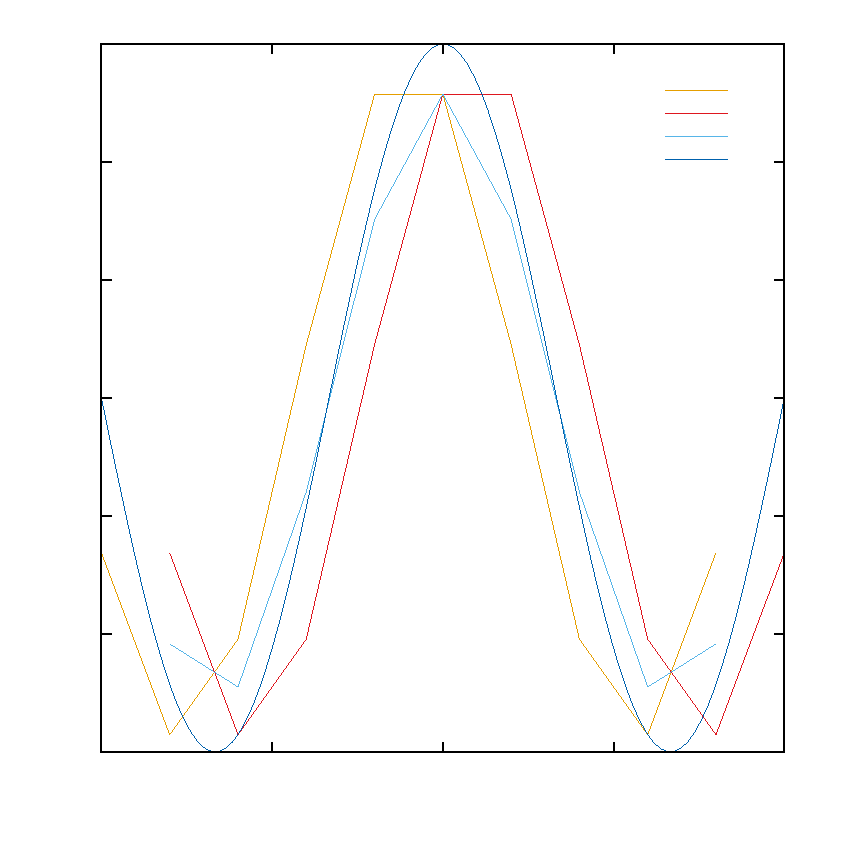
\includegraphics{1stcos10}}%
    \gplfronttext
  \end{picture}%
\endgroup

			\caption{Comparison of numerical differentiation of cos$(3x)$ using 10 intervals}
		\end{figure}
		\begin{figure}
			\centering
			% GNUPLOT: LaTeX picture with Postscript
\begingroup
  \makeatletter
  \providecommand\color[2][]{%
    \GenericError{(gnuplot) \space\space\space\@spaces}{%
      Package color not loaded in conjunction with
      terminal option `colourtext'%
    }{See the gnuplot documentation for explanation.%
    }{Either use 'blacktext' in gnuplot or load the package
      color.sty in LaTeX.}%
    \renewcommand\color[2][]{}%
  }%
  \providecommand\includegraphics[2][]{%
    \GenericError{(gnuplot) \space\space\space\@spaces}{%
      Package graphicx or graphics not loaded%
    }{See the gnuplot documentation for explanation.%
    }{The gnuplot epslatex terminal needs graphicx.sty or graphics.sty.}%
    \renewcommand\includegraphics[2][]{}%
  }%
  \providecommand\rotatebox[2]{#2}%
  \@ifundefined{ifGPcolor}{%
    \newif\ifGPcolor
    \GPcolortrue
  }{}%
  \@ifundefined{ifGPblacktext}{%
    \newif\ifGPblacktext
    \GPblacktextfalse
  }{}%
  % define a \g@addto@macro without @ in the name:
  \let\gplgaddtomacro\g@addto@macro
  % define empty templates for all commands taking text:
  \gdef\gplbacktext{}%
  \gdef\gplfronttext{}%
  \makeatother
  \ifGPblacktext
    % no textcolor at all
    \def\colorrgb#1{}%
    \def\colorgray#1{}%
  \else
    % gray or color?
    \ifGPcolor
      \def\colorrgb#1{\color[rgb]{#1}}%
      \def\colorgray#1{\color[gray]{#1}}%
      \expandafter\def\csname LTw\endcsname{\color{white}}%
      \expandafter\def\csname LTb\endcsname{\color{black}}%
      \expandafter\def\csname LTa\endcsname{\color{black}}%
      \expandafter\def\csname LT0\endcsname{\color[rgb]{1,0,0}}%
      \expandafter\def\csname LT1\endcsname{\color[rgb]{0,1,0}}%
      \expandafter\def\csname LT2\endcsname{\color[rgb]{0,0,1}}%
      \expandafter\def\csname LT3\endcsname{\color[rgb]{1,0,1}}%
      \expandafter\def\csname LT4\endcsname{\color[rgb]{0,1,1}}%
      \expandafter\def\csname LT5\endcsname{\color[rgb]{1,1,0}}%
      \expandafter\def\csname LT6\endcsname{\color[rgb]{0,0,0}}%
      \expandafter\def\csname LT7\endcsname{\color[rgb]{1,0.3,0}}%
      \expandafter\def\csname LT8\endcsname{\color[rgb]{0.5,0.5,0.5}}%
    \else
      % gray
      \def\colorrgb#1{\color{black}}%
      \def\colorgray#1{\color[gray]{#1}}%
      \expandafter\def\csname LTw\endcsname{\color{white}}%
      \expandafter\def\csname LTb\endcsname{\color{black}}%
      \expandafter\def\csname LTa\endcsname{\color{black}}%
      \expandafter\def\csname LT0\endcsname{\color{black}}%
      \expandafter\def\csname LT1\endcsname{\color{black}}%
      \expandafter\def\csname LT2\endcsname{\color{black}}%
      \expandafter\def\csname LT3\endcsname{\color{black}}%
      \expandafter\def\csname LT4\endcsname{\color{black}}%
      \expandafter\def\csname LT5\endcsname{\color{black}}%
      \expandafter\def\csname LT6\endcsname{\color{black}}%
      \expandafter\def\csname LT7\endcsname{\color{black}}%
      \expandafter\def\csname LT8\endcsname{\color{black}}%
    \fi
  \fi
    \setlength{\unitlength}{0.0500bp}%
    \ifx\gptboxheight\undefined%
      \newlength{\gptboxheight}%
      \newlength{\gptboxwidth}%
      \newsavebox{\gptboxtext}%
    \fi%
    \setlength{\fboxrule}{0.5pt}%
    \setlength{\fboxsep}{1pt}%
\begin{picture}(7766.00,7766.00)%
    \gplgaddtomacro\gplbacktext{%
      \csname LTb\endcsname%
      \put(682,704){\makebox(0,0)[r]{\strut{}$-3$}}%
      \put(682,1837){\makebox(0,0)[r]{\strut{}$-2$}}%
      \put(682,2970){\makebox(0,0)[r]{\strut{}$-1$}}%
      \put(682,4102){\makebox(0,0)[r]{\strut{}$0$}}%
      \put(682,5235){\makebox(0,0)[r]{\strut{}$1$}}%
      \put(682,6368){\makebox(0,0)[r]{\strut{}$2$}}%
      \put(682,7501){\makebox(0,0)[r]{\strut{}$3$}}%
      \put(814,484){\makebox(0,0){\strut{}$0$}}%
      \put(2453,484){\makebox(0,0){\strut{}$\pi/4$}}%
      \put(4091,484){\makebox(0,0){\strut{}$\pi/2$}}%
      \put(5730,484){\makebox(0,0){\strut{}$3\pi/4$}}%
      \put(7369,484){\makebox(0,0){\strut{}$\pi$}}%
    }%
    \gplgaddtomacro\gplfronttext{%
      \csname LTb\endcsname%
      \put(176,4102){\rotatebox{-270}{\makebox(0,0){\strut{}$f(x)$}}}%
      \put(4091,154){\makebox(0,0){\strut{}$x$}}%
      \csname LTb\endcsname%
      \put(6097,7051){\makebox(0,0)[r]{\strut{}Forward}}%
      \csname LTb\endcsname%
      \put(6097,6831){\makebox(0,0)[r]{\strut{}Backward}}%
      \csname LTb\endcsname%
      \put(6097,6611){\makebox(0,0)[r]{\strut{}Central}}%
      \csname LTb\endcsname%
      \put(6097,6391){\makebox(0,0)[r]{\strut{}Analytical}}%
    }%
    \gplbacktext
    \put(0,0){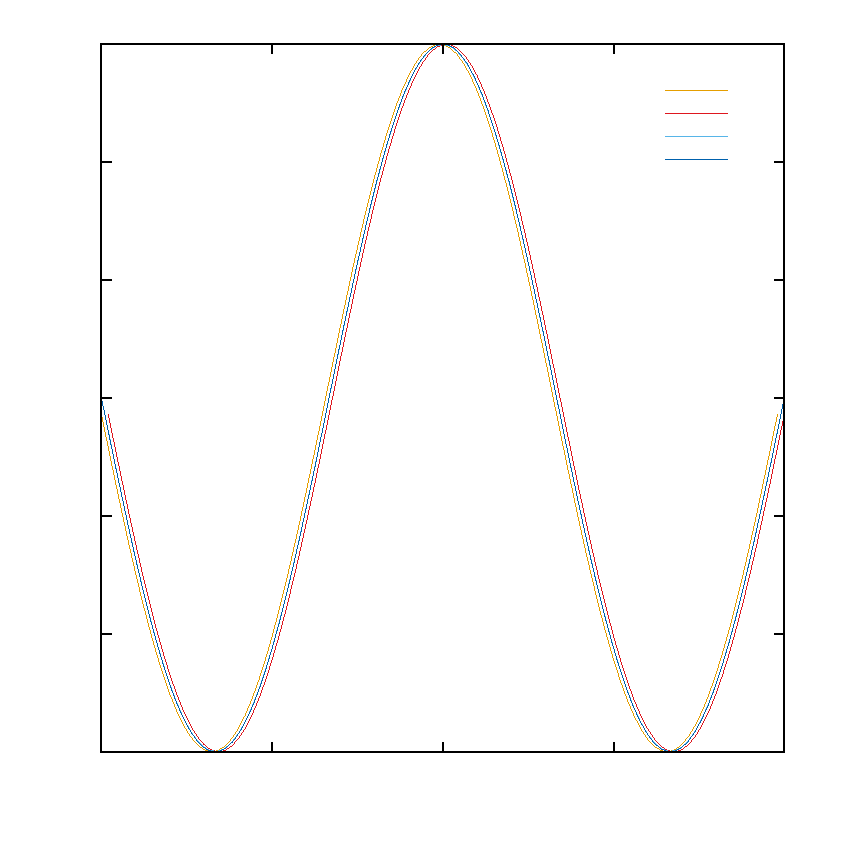
\includegraphics{1stcos100}}%
    \gplfronttext
  \end{picture}%
\endgroup

			\caption{Comparison of numerical differentiation of cos$(3x)$ using 100 intervals}
		\end{figure}

		\section*{2nd order numerical differentiation}
		Another algorithm was coded in C++ for double derivatives using similar three commonly used schemes. The functions sin$(3x)$ and cos$(3x)$ were differentiated twice using forward difference method, backward difference method and central difference method.
		
		\subsection*{Forward difference method for 2nd derivative}
		\begin{equation}
		f^\prime(x) = \frac{f(x_{i+2})-2f(x_{i+1})+f(x_i)}{h^2}
		\end{equation}
		
		\subsection*{Backward difference method for 2nd derivative}
		\begin{equation}
		f^\prime(x) = \frac{f(x_i)-2f(x_{i-1})+f(x_{i-2})}{h^2}
		\end{equation}
		
		\subsection*{Central difference method for 2nd derivative}
		\begin{equation}
		f^\prime(x) = \frac{f(x_{i+1})-2f(x)+f(x_{i-1})}{h^2}
		\end{equation}
		
		The results are shown in the figures below.

		\begin{figure}
			\centering
			% GNUPLOT: LaTeX picture with Postscript
\begingroup
  \makeatletter
  \providecommand\color[2][]{%
    \GenericError{(gnuplot) \space\space\space\@spaces}{%
      Package color not loaded in conjunction with
      terminal option `colourtext'%
    }{See the gnuplot documentation for explanation.%
    }{Either use 'blacktext' in gnuplot or load the package
      color.sty in LaTeX.}%
    \renewcommand\color[2][]{}%
  }%
  \providecommand\includegraphics[2][]{%
    \GenericError{(gnuplot) \space\space\space\@spaces}{%
      Package graphicx or graphics not loaded%
    }{See the gnuplot documentation for explanation.%
    }{The gnuplot epslatex terminal needs graphicx.sty or graphics.sty.}%
    \renewcommand\includegraphics[2][]{}%
  }%
  \providecommand\rotatebox[2]{#2}%
  \@ifundefined{ifGPcolor}{%
    \newif\ifGPcolor
    \GPcolortrue
  }{}%
  \@ifundefined{ifGPblacktext}{%
    \newif\ifGPblacktext
    \GPblacktextfalse
  }{}%
  % define a \g@addto@macro without @ in the name:
  \let\gplgaddtomacro\g@addto@macro
  % define empty templates for all commands taking text:
  \gdef\gplbacktext{}%
  \gdef\gplfronttext{}%
  \makeatother
  \ifGPblacktext
    % no textcolor at all
    \def\colorrgb#1{}%
    \def\colorgray#1{}%
  \else
    % gray or color?
    \ifGPcolor
      \def\colorrgb#1{\color[rgb]{#1}}%
      \def\colorgray#1{\color[gray]{#1}}%
      \expandafter\def\csname LTw\endcsname{\color{white}}%
      \expandafter\def\csname LTb\endcsname{\color{black}}%
      \expandafter\def\csname LTa\endcsname{\color{black}}%
      \expandafter\def\csname LT0\endcsname{\color[rgb]{1,0,0}}%
      \expandafter\def\csname LT1\endcsname{\color[rgb]{0,1,0}}%
      \expandafter\def\csname LT2\endcsname{\color[rgb]{0,0,1}}%
      \expandafter\def\csname LT3\endcsname{\color[rgb]{1,0,1}}%
      \expandafter\def\csname LT4\endcsname{\color[rgb]{0,1,1}}%
      \expandafter\def\csname LT5\endcsname{\color[rgb]{1,1,0}}%
      \expandafter\def\csname LT6\endcsname{\color[rgb]{0,0,0}}%
      \expandafter\def\csname LT7\endcsname{\color[rgb]{1,0.3,0}}%
      \expandafter\def\csname LT8\endcsname{\color[rgb]{0.5,0.5,0.5}}%
    \else
      % gray
      \def\colorrgb#1{\color{black}}%
      \def\colorgray#1{\color[gray]{#1}}%
      \expandafter\def\csname LTw\endcsname{\color{white}}%
      \expandafter\def\csname LTb\endcsname{\color{black}}%
      \expandafter\def\csname LTa\endcsname{\color{black}}%
      \expandafter\def\csname LT0\endcsname{\color{black}}%
      \expandafter\def\csname LT1\endcsname{\color{black}}%
      \expandafter\def\csname LT2\endcsname{\color{black}}%
      \expandafter\def\csname LT3\endcsname{\color{black}}%
      \expandafter\def\csname LT4\endcsname{\color{black}}%
      \expandafter\def\csname LT5\endcsname{\color{black}}%
      \expandafter\def\csname LT6\endcsname{\color{black}}%
      \expandafter\def\csname LT7\endcsname{\color{black}}%
      \expandafter\def\csname LT8\endcsname{\color{black}}%
    \fi
  \fi
    \setlength{\unitlength}{0.0500bp}%
    \ifx\gptboxheight\undefined%
      \newlength{\gptboxheight}%
      \newlength{\gptboxwidth}%
      \newsavebox{\gptboxtext}%
    \fi%
    \setlength{\fboxrule}{0.5pt}%
    \setlength{\fboxsep}{1pt}%
\begin{picture}(7766.00,7766.00)%
    \gplgaddtomacro\gplbacktext{%
      \csname LTb\endcsname%
      \put(814,704){\makebox(0,0)[r]{\strut{}$-10$}}%
      \put(814,1384){\makebox(0,0)[r]{\strut{}$-8$}}%
      \put(814,2063){\makebox(0,0)[r]{\strut{}$-6$}}%
      \put(814,2743){\makebox(0,0)[r]{\strut{}$-4$}}%
      \put(814,3423){\makebox(0,0)[r]{\strut{}$-2$}}%
      \put(814,4103){\makebox(0,0)[r]{\strut{}$0$}}%
      \put(814,4782){\makebox(0,0)[r]{\strut{}$2$}}%
      \put(814,5462){\makebox(0,0)[r]{\strut{}$4$}}%
      \put(814,6142){\makebox(0,0)[r]{\strut{}$6$}}%
      \put(814,6821){\makebox(0,0)[r]{\strut{}$8$}}%
      \put(814,7501){\makebox(0,0)[r]{\strut{}$10$}}%
      \put(946,484){\makebox(0,0){\strut{}$0$}}%
      \put(2583,484){\makebox(0,0){\strut{}$\pi/4$}}%
      \put(4220,484){\makebox(0,0){\strut{}$\pi/2$}}%
      \put(5858,484){\makebox(0,0){\strut{}$3\pi/4$}}%
    }%
    \gplgaddtomacro\gplfronttext{%
      \csname LTb\endcsname%
      \put(176,4102){\rotatebox{-270}{\makebox(0,0){\strut{}$f(x)$}}}%
      \put(3893,154){\makebox(0,0){\strut{}$x$}}%
      \csname LTb\endcsname%
      \put(6431,6949){\makebox(0,0)[r]{\strut{}Forward}}%
      \csname LTb\endcsname%
      \put(6431,6729){\makebox(0,0)[r]{\strut{}Backward}}%
      \csname LTb\endcsname%
      \put(6431,6509){\makebox(0,0)[r]{\strut{}Central}}%
      \csname LTb\endcsname%
      \put(6431,6289){\makebox(0,0)[r]{\strut{}Analytical}}%
    }%
    \gplbacktext
    \put(0,0){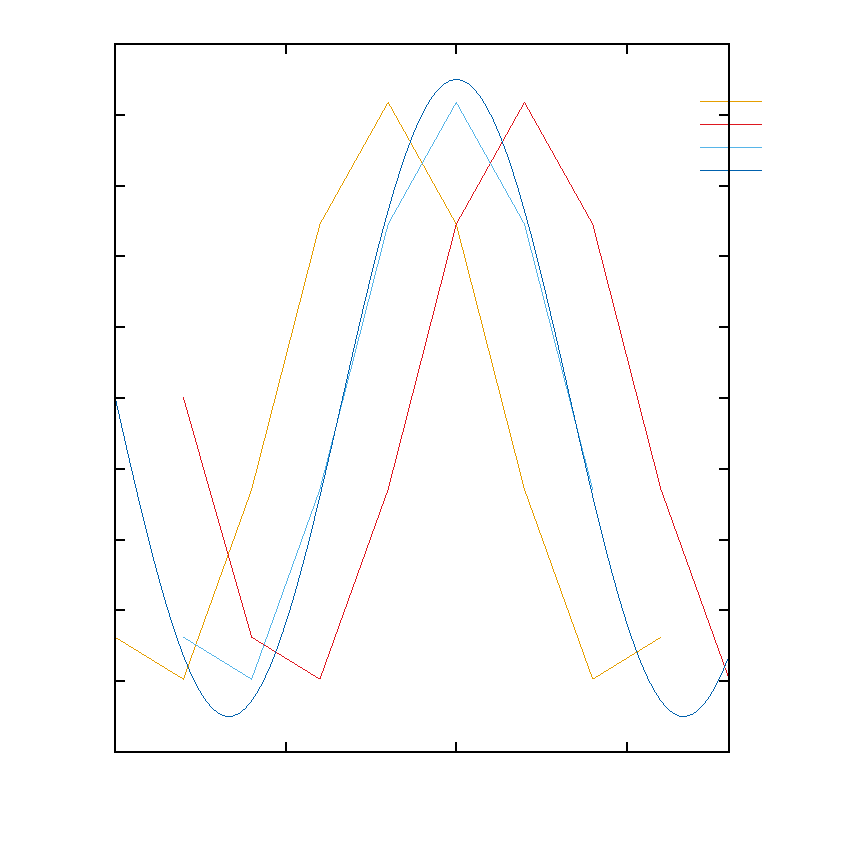
\includegraphics{2ndsin10}}%
    \gplfronttext
  \end{picture}%
\endgroup

			\caption{Comparison of double derivative of sin$(3x)$ using 10 intervals}
		\end{figure}
		\begin{figure}
			\centering
			% GNUPLOT: LaTeX picture with Postscript
\begingroup
  \makeatletter
  \providecommand\color[2][]{%
    \GenericError{(gnuplot) \space\space\space\@spaces}{%
      Package color not loaded in conjunction with
      terminal option `colourtext'%
    }{See the gnuplot documentation for explanation.%
    }{Either use 'blacktext' in gnuplot or load the package
      color.sty in LaTeX.}%
    \renewcommand\color[2][]{}%
  }%
  \providecommand\includegraphics[2][]{%
    \GenericError{(gnuplot) \space\space\space\@spaces}{%
      Package graphicx or graphics not loaded%
    }{See the gnuplot documentation for explanation.%
    }{The gnuplot epslatex terminal needs graphicx.sty or graphics.sty.}%
    \renewcommand\includegraphics[2][]{}%
  }%
  \providecommand\rotatebox[2]{#2}%
  \@ifundefined{ifGPcolor}{%
    \newif\ifGPcolor
    \GPcolortrue
  }{}%
  \@ifundefined{ifGPblacktext}{%
    \newif\ifGPblacktext
    \GPblacktextfalse
  }{}%
  % define a \g@addto@macro without @ in the name:
  \let\gplgaddtomacro\g@addto@macro
  % define empty templates for all commands taking text:
  \gdef\gplbacktext{}%
  \gdef\gplfronttext{}%
  \makeatother
  \ifGPblacktext
    % no textcolor at all
    \def\colorrgb#1{}%
    \def\colorgray#1{}%
  \else
    % gray or color?
    \ifGPcolor
      \def\colorrgb#1{\color[rgb]{#1}}%
      \def\colorgray#1{\color[gray]{#1}}%
      \expandafter\def\csname LTw\endcsname{\color{white}}%
      \expandafter\def\csname LTb\endcsname{\color{black}}%
      \expandafter\def\csname LTa\endcsname{\color{black}}%
      \expandafter\def\csname LT0\endcsname{\color[rgb]{1,0,0}}%
      \expandafter\def\csname LT1\endcsname{\color[rgb]{0,1,0}}%
      \expandafter\def\csname LT2\endcsname{\color[rgb]{0,0,1}}%
      \expandafter\def\csname LT3\endcsname{\color[rgb]{1,0,1}}%
      \expandafter\def\csname LT4\endcsname{\color[rgb]{0,1,1}}%
      \expandafter\def\csname LT5\endcsname{\color[rgb]{1,1,0}}%
      \expandafter\def\csname LT6\endcsname{\color[rgb]{0,0,0}}%
      \expandafter\def\csname LT7\endcsname{\color[rgb]{1,0.3,0}}%
      \expandafter\def\csname LT8\endcsname{\color[rgb]{0.5,0.5,0.5}}%
    \else
      % gray
      \def\colorrgb#1{\color{black}}%
      \def\colorgray#1{\color[gray]{#1}}%
      \expandafter\def\csname LTw\endcsname{\color{white}}%
      \expandafter\def\csname LTb\endcsname{\color{black}}%
      \expandafter\def\csname LTa\endcsname{\color{black}}%
      \expandafter\def\csname LT0\endcsname{\color{black}}%
      \expandafter\def\csname LT1\endcsname{\color{black}}%
      \expandafter\def\csname LT2\endcsname{\color{black}}%
      \expandafter\def\csname LT3\endcsname{\color{black}}%
      \expandafter\def\csname LT4\endcsname{\color{black}}%
      \expandafter\def\csname LT5\endcsname{\color{black}}%
      \expandafter\def\csname LT6\endcsname{\color{black}}%
      \expandafter\def\csname LT7\endcsname{\color{black}}%
      \expandafter\def\csname LT8\endcsname{\color{black}}%
    \fi
  \fi
    \setlength{\unitlength}{0.0500bp}%
    \ifx\gptboxheight\undefined%
      \newlength{\gptboxheight}%
      \newlength{\gptboxwidth}%
      \newsavebox{\gptboxtext}%
    \fi%
    \setlength{\fboxrule}{0.5pt}%
    \setlength{\fboxsep}{1pt}%
\begin{picture}(7766.00,7766.00)%
    \gplgaddtomacro\gplbacktext{%
      \csname LTb\endcsname%
      \put(814,704){\makebox(0,0)[r]{\strut{}$-10$}}%
      \put(814,1384){\makebox(0,0)[r]{\strut{}$-8$}}%
      \put(814,2063){\makebox(0,0)[r]{\strut{}$-6$}}%
      \put(814,2743){\makebox(0,0)[r]{\strut{}$-4$}}%
      \put(814,3423){\makebox(0,0)[r]{\strut{}$-2$}}%
      \put(814,4103){\makebox(0,0)[r]{\strut{}$0$}}%
      \put(814,4782){\makebox(0,0)[r]{\strut{}$2$}}%
      \put(814,5462){\makebox(0,0)[r]{\strut{}$4$}}%
      \put(814,6142){\makebox(0,0)[r]{\strut{}$6$}}%
      \put(814,6821){\makebox(0,0)[r]{\strut{}$8$}}%
      \put(814,7501){\makebox(0,0)[r]{\strut{}$10$}}%
      \put(946,484){\makebox(0,0){\strut{}$0$}}%
      \put(2568,484){\makebox(0,0){\strut{}$\pi/4$}}%
      \put(4190,484){\makebox(0,0){\strut{}$\pi/2$}}%
      \put(5812,484){\makebox(0,0){\strut{}$3\pi/4$}}%
    }%
    \gplgaddtomacro\gplfronttext{%
      \csname LTb\endcsname%
      \put(176,4102){\rotatebox{-270}{\makebox(0,0){\strut{}$f(x)$}}}%
      \put(4157,154){\makebox(0,0){\strut{}$x$}}%
      \csname LTb\endcsname%
      \put(6372,6949){\makebox(0,0)[r]{\strut{}Forward}}%
      \csname LTb\endcsname%
      \put(6372,6729){\makebox(0,0)[r]{\strut{}Backward}}%
      \csname LTb\endcsname%
      \put(6372,6509){\makebox(0,0)[r]{\strut{}Central}}%
      \csname LTb\endcsname%
      \put(6372,6289){\makebox(0,0)[r]{\strut{}Analytical}}%
    }%
    \gplbacktext
    \put(0,0){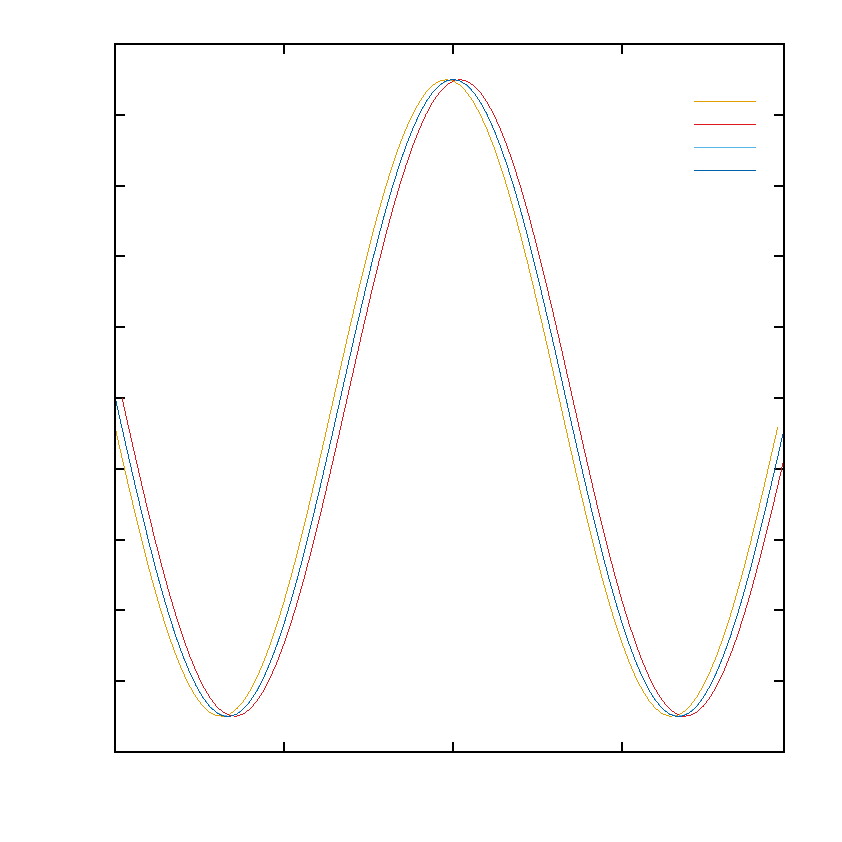
\includegraphics{2ndsin100}}%
    \gplfronttext
  \end{picture}%
\endgroup

			\caption{Comparison of double derivative of sin$(3x)$ using 100 intervals}
		\end{figure}
		\begin{figure}
			\centering
			% GNUPLOT: LaTeX picture with Postscript
\begingroup
  \makeatletter
  \providecommand\color[2][]{%
    \GenericError{(gnuplot) \space\space\space\@spaces}{%
      Package color not loaded in conjunction with
      terminal option `colourtext'%
    }{See the gnuplot documentation for explanation.%
    }{Either use 'blacktext' in gnuplot or load the package
      color.sty in LaTeX.}%
    \renewcommand\color[2][]{}%
  }%
  \providecommand\includegraphics[2][]{%
    \GenericError{(gnuplot) \space\space\space\@spaces}{%
      Package graphicx or graphics not loaded%
    }{See the gnuplot documentation for explanation.%
    }{The gnuplot epslatex terminal needs graphicx.sty or graphics.sty.}%
    \renewcommand\includegraphics[2][]{}%
  }%
  \providecommand\rotatebox[2]{#2}%
  \@ifundefined{ifGPcolor}{%
    \newif\ifGPcolor
    \GPcolortrue
  }{}%
  \@ifundefined{ifGPblacktext}{%
    \newif\ifGPblacktext
    \GPblacktextfalse
  }{}%
  % define a \g@addto@macro without @ in the name:
  \let\gplgaddtomacro\g@addto@macro
  % define empty templates for all commands taking text:
  \gdef\gplbacktext{}%
  \gdef\gplfronttext{}%
  \makeatother
  \ifGPblacktext
    % no textcolor at all
    \def\colorrgb#1{}%
    \def\colorgray#1{}%
  \else
    % gray or color?
    \ifGPcolor
      \def\colorrgb#1{\color[rgb]{#1}}%
      \def\colorgray#1{\color[gray]{#1}}%
      \expandafter\def\csname LTw\endcsname{\color{white}}%
      \expandafter\def\csname LTb\endcsname{\color{black}}%
      \expandafter\def\csname LTa\endcsname{\color{black}}%
      \expandafter\def\csname LT0\endcsname{\color[rgb]{1,0,0}}%
      \expandafter\def\csname LT1\endcsname{\color[rgb]{0,1,0}}%
      \expandafter\def\csname LT2\endcsname{\color[rgb]{0,0,1}}%
      \expandafter\def\csname LT3\endcsname{\color[rgb]{1,0,1}}%
      \expandafter\def\csname LT4\endcsname{\color[rgb]{0,1,1}}%
      \expandafter\def\csname LT5\endcsname{\color[rgb]{1,1,0}}%
      \expandafter\def\csname LT6\endcsname{\color[rgb]{0,0,0}}%
      \expandafter\def\csname LT7\endcsname{\color[rgb]{1,0.3,0}}%
      \expandafter\def\csname LT8\endcsname{\color[rgb]{0.5,0.5,0.5}}%
    \else
      % gray
      \def\colorrgb#1{\color{black}}%
      \def\colorgray#1{\color[gray]{#1}}%
      \expandafter\def\csname LTw\endcsname{\color{white}}%
      \expandafter\def\csname LTb\endcsname{\color{black}}%
      \expandafter\def\csname LTa\endcsname{\color{black}}%
      \expandafter\def\csname LT0\endcsname{\color{black}}%
      \expandafter\def\csname LT1\endcsname{\color{black}}%
      \expandafter\def\csname LT2\endcsname{\color{black}}%
      \expandafter\def\csname LT3\endcsname{\color{black}}%
      \expandafter\def\csname LT4\endcsname{\color{black}}%
      \expandafter\def\csname LT5\endcsname{\color{black}}%
      \expandafter\def\csname LT6\endcsname{\color{black}}%
      \expandafter\def\csname LT7\endcsname{\color{black}}%
      \expandafter\def\csname LT8\endcsname{\color{black}}%
    \fi
  \fi
    \setlength{\unitlength}{0.0500bp}%
    \ifx\gptboxheight\undefined%
      \newlength{\gptboxheight}%
      \newlength{\gptboxwidth}%
      \newsavebox{\gptboxtext}%
    \fi%
    \setlength{\fboxrule}{0.5pt}%
    \setlength{\fboxsep}{1pt}%
\begin{picture}(7766.00,7766.00)%
    \gplgaddtomacro\gplbacktext{%
      \csname LTb\endcsname%
      \put(814,704){\makebox(0,0)[r]{\strut{}$-10$}}%
      \put(814,1384){\makebox(0,0)[r]{\strut{}$-8$}}%
      \put(814,2063){\makebox(0,0)[r]{\strut{}$-6$}}%
      \put(814,2743){\makebox(0,0)[r]{\strut{}$-4$}}%
      \put(814,3423){\makebox(0,0)[r]{\strut{}$-2$}}%
      \put(814,4103){\makebox(0,0)[r]{\strut{}$0$}}%
      \put(814,4782){\makebox(0,0)[r]{\strut{}$2$}}%
      \put(814,5462){\makebox(0,0)[r]{\strut{}$4$}}%
      \put(814,6142){\makebox(0,0)[r]{\strut{}$6$}}%
      \put(814,6821){\makebox(0,0)[r]{\strut{}$8$}}%
      \put(814,7501){\makebox(0,0)[r]{\strut{}$10$}}%
      \put(946,484){\makebox(0,0){\strut{}$0$}}%
      \put(2583,484){\makebox(0,0){\strut{}$\pi/4$}}%
      \put(4220,484){\makebox(0,0){\strut{}$\pi/2$}}%
      \put(5858,484){\makebox(0,0){\strut{}$3\pi/4$}}%
    }%
    \gplgaddtomacro\gplfronttext{%
      \csname LTb\endcsname%
      \put(176,4102){\rotatebox{-270}{\makebox(0,0){\strut{}$f(x)$}}}%
      \put(3893,154){\makebox(0,0){\strut{}$x$}}%
      \csname LTb\endcsname%
      \put(5806,6949){\makebox(0,0)[r]{\strut{}Forward}}%
      \csname LTb\endcsname%
      \put(5806,6729){\makebox(0,0)[r]{\strut{}Backward}}%
      \csname LTb\endcsname%
      \put(5806,6509){\makebox(0,0)[r]{\strut{}Central}}%
      \csname LTb\endcsname%
      \put(5806,6289){\makebox(0,0)[r]{\strut{}Analytical}}%
    }%
    \gplbacktext
    \put(0,0){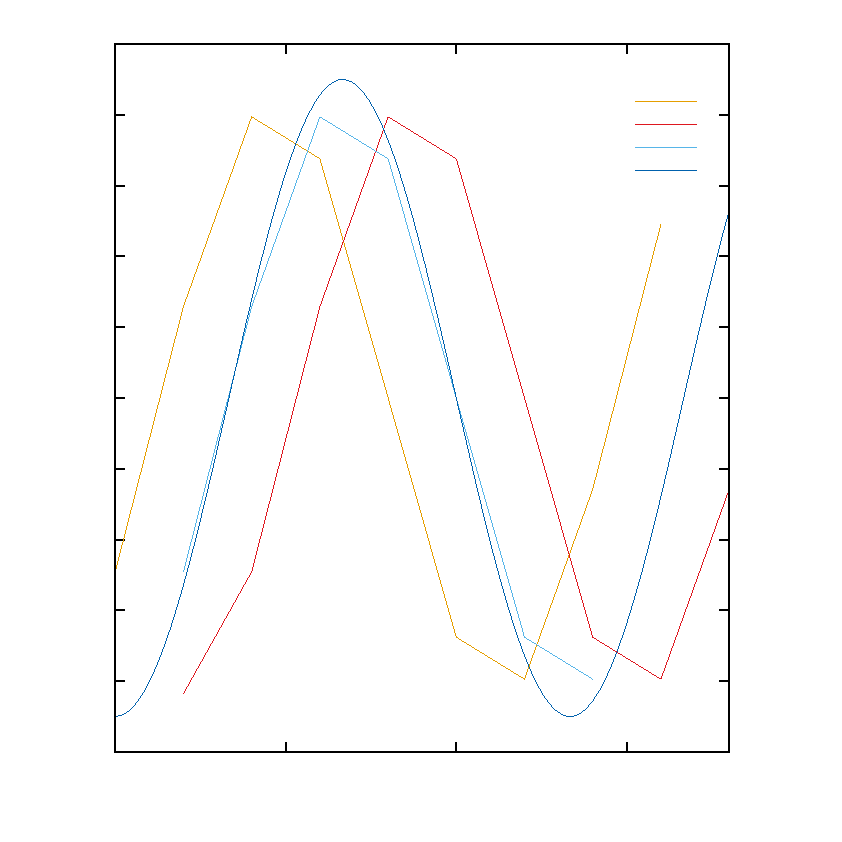
\includegraphics{2ndcos10}}%
    \gplfronttext
  \end{picture}%
\endgroup

			\caption{Comparison of double derivative of cos$(3x)$ using 10 intervals}
		\end{figure}
		\begin{figure}
			\centering
			% GNUPLOT: LaTeX picture with Postscript
\begingroup
  \makeatletter
  \providecommand\color[2][]{%
    \GenericError{(gnuplot) \space\space\space\@spaces}{%
      Package color not loaded in conjunction with
      terminal option `colourtext'%
    }{See the gnuplot documentation for explanation.%
    }{Either use 'blacktext' in gnuplot or load the package
      color.sty in LaTeX.}%
    \renewcommand\color[2][]{}%
  }%
  \providecommand\includegraphics[2][]{%
    \GenericError{(gnuplot) \space\space\space\@spaces}{%
      Package graphicx or graphics not loaded%
    }{See the gnuplot documentation for explanation.%
    }{The gnuplot epslatex terminal needs graphicx.sty or graphics.sty.}%
    \renewcommand\includegraphics[2][]{}%
  }%
  \providecommand\rotatebox[2]{#2}%
  \@ifundefined{ifGPcolor}{%
    \newif\ifGPcolor
    \GPcolortrue
  }{}%
  \@ifundefined{ifGPblacktext}{%
    \newif\ifGPblacktext
    \GPblacktextfalse
  }{}%
  % define a \g@addto@macro without @ in the name:
  \let\gplgaddtomacro\g@addto@macro
  % define empty templates for all commands taking text:
  \gdef\gplbacktext{}%
  \gdef\gplfronttext{}%
  \makeatother
  \ifGPblacktext
    % no textcolor at all
    \def\colorrgb#1{}%
    \def\colorgray#1{}%
  \else
    % gray or color?
    \ifGPcolor
      \def\colorrgb#1{\color[rgb]{#1}}%
      \def\colorgray#1{\color[gray]{#1}}%
      \expandafter\def\csname LTw\endcsname{\color{white}}%
      \expandafter\def\csname LTb\endcsname{\color{black}}%
      \expandafter\def\csname LTa\endcsname{\color{black}}%
      \expandafter\def\csname LT0\endcsname{\color[rgb]{1,0,0}}%
      \expandafter\def\csname LT1\endcsname{\color[rgb]{0,1,0}}%
      \expandafter\def\csname LT2\endcsname{\color[rgb]{0,0,1}}%
      \expandafter\def\csname LT3\endcsname{\color[rgb]{1,0,1}}%
      \expandafter\def\csname LT4\endcsname{\color[rgb]{0,1,1}}%
      \expandafter\def\csname LT5\endcsname{\color[rgb]{1,1,0}}%
      \expandafter\def\csname LT6\endcsname{\color[rgb]{0,0,0}}%
      \expandafter\def\csname LT7\endcsname{\color[rgb]{1,0.3,0}}%
      \expandafter\def\csname LT8\endcsname{\color[rgb]{0.5,0.5,0.5}}%
    \else
      % gray
      \def\colorrgb#1{\color{black}}%
      \def\colorgray#1{\color[gray]{#1}}%
      \expandafter\def\csname LTw\endcsname{\color{white}}%
      \expandafter\def\csname LTb\endcsname{\color{black}}%
      \expandafter\def\csname LTa\endcsname{\color{black}}%
      \expandafter\def\csname LT0\endcsname{\color{black}}%
      \expandafter\def\csname LT1\endcsname{\color{black}}%
      \expandafter\def\csname LT2\endcsname{\color{black}}%
      \expandafter\def\csname LT3\endcsname{\color{black}}%
      \expandafter\def\csname LT4\endcsname{\color{black}}%
      \expandafter\def\csname LT5\endcsname{\color{black}}%
      \expandafter\def\csname LT6\endcsname{\color{black}}%
      \expandafter\def\csname LT7\endcsname{\color{black}}%
      \expandafter\def\csname LT8\endcsname{\color{black}}%
    \fi
  \fi
    \setlength{\unitlength}{0.0500bp}%
    \ifx\gptboxheight\undefined%
      \newlength{\gptboxheight}%
      \newlength{\gptboxwidth}%
      \newsavebox{\gptboxtext}%
    \fi%
    \setlength{\fboxrule}{0.5pt}%
    \setlength{\fboxsep}{1pt}%
\begin{picture}(7766.00,7766.00)%
    \gplgaddtomacro\gplbacktext{%
      \csname LTb\endcsname%
      \put(814,704){\makebox(0,0)[r]{\strut{}$-10$}}%
      \put(814,1384){\makebox(0,0)[r]{\strut{}$-8$}}%
      \put(814,2063){\makebox(0,0)[r]{\strut{}$-6$}}%
      \put(814,2743){\makebox(0,0)[r]{\strut{}$-4$}}%
      \put(814,3423){\makebox(0,0)[r]{\strut{}$-2$}}%
      \put(814,4103){\makebox(0,0)[r]{\strut{}$0$}}%
      \put(814,4782){\makebox(0,0)[r]{\strut{}$2$}}%
      \put(814,5462){\makebox(0,0)[r]{\strut{}$4$}}%
      \put(814,6142){\makebox(0,0)[r]{\strut{}$6$}}%
      \put(814,6821){\makebox(0,0)[r]{\strut{}$8$}}%
      \put(814,7501){\makebox(0,0)[r]{\strut{}$10$}}%
      \put(946,484){\makebox(0,0){\strut{}$0$}}%
      \put(2568,484){\makebox(0,0){\strut{}$\pi/4$}}%
      \put(4190,484){\makebox(0,0){\strut{}$\pi/2$}}%
      \put(5812,484){\makebox(0,0){\strut{}$3\pi/4$}}%
    }%
    \gplgaddtomacro\gplfronttext{%
      \csname LTb\endcsname%
      \put(176,4102){\rotatebox{-270}{\makebox(0,0){\strut{}$f(x)$}}}%
      \put(4157,154){\makebox(0,0){\strut{}$x$}}%
      \csname LTb\endcsname%
      \put(5753,6949){\makebox(0,0)[r]{\strut{}Forward}}%
      \csname LTb\endcsname%
      \put(5753,6729){\makebox(0,0)[r]{\strut{}Backward}}%
      \csname LTb\endcsname%
      \put(5753,6509){\makebox(0,0)[r]{\strut{}Central}}%
      \csname LTb\endcsname%
      \put(5753,6289){\makebox(0,0)[r]{\strut{}Analytical}}%
    }%
    \gplbacktext
    \put(0,0){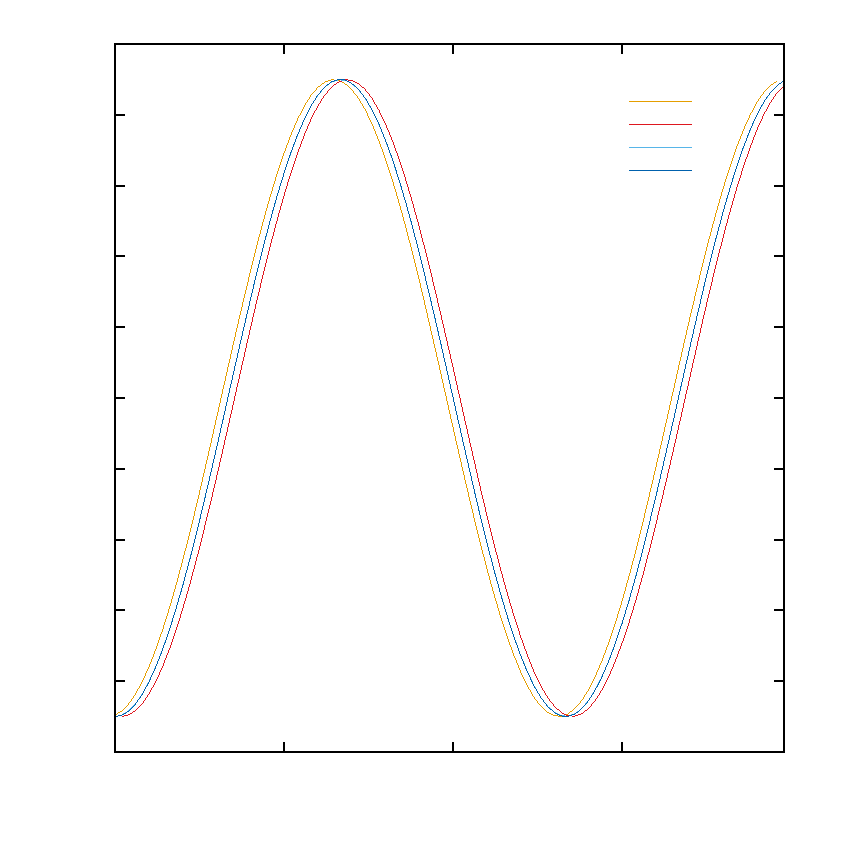
\includegraphics{2ndcos100}}%
    \gplfronttext
  \end{picture}%
\endgroup

			\caption{Comparison of double derivative of cos$(3x)$ using 100 intervals}
		\end{figure}
\end{document}